\documentclass{article}

\usepackage{pythontex}
\usepackage{graphicx}

\usepackage{url}

\newcommand{\pymultiply}[2]{\py{#1*#2}}

\begin{document}

\begin{pycode}
print("Python says ``Hello!''")
\end{pycode}

$8 \times 256 = \pymultiply{8}{256}$

\section{Creating a chart}
\begin{pylabblock}
from matplotlib import pyplot as plt
import numpy as np
plt.rc('text', usetex=True)
plt.rc('font', family='serif')
plt.rc('font', size=10.0)
plt.rc('legend', fontsize=10.0)
plt.rc('font', weight='normal')

x = np.linspace(0, 10)
y = np.sin(x)+2

plt.figure(figsize=(4, 2.5))
plt.plot(x, y, label='$\sin(x)$')

plt.xlabel(r'$x\mathrm{-axis}$')
plt.ylabel(r'$y\mathrm{-axis}$')
plt.legend(loc='lower right')
plt.savefig('myplot.pdf', bbox_inches='tight')
\end{pylabblock}

\begin{center}
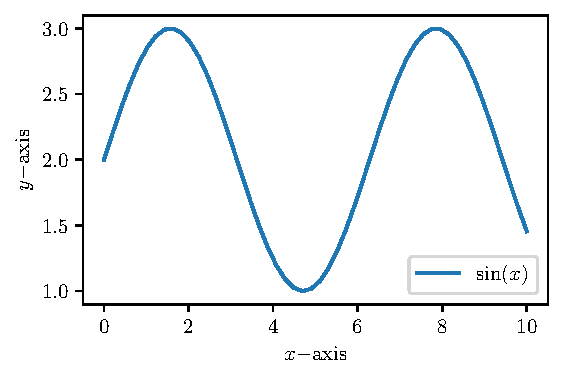
\includegraphics{myplot.pdf}
\end{center}

\section{Save chart in excel}
\begin{pylabblock}
from datetime import date

from openpyxl import Workbook
from openpyxl.chart import LineChart,Reference
from openpyxl.chart.axis import DateAxis

wb = Workbook()
ws = wb.active

for idx, value in enumerate(x, 1):
    ws.append([value, f"=SIN(A{idx})+2"])

c1 = LineChart()

data = Reference(ws, min_col=2, min_row=1, max_col=2, max_row=len(y))
c1.add_data(data)

ws.add_chart(c1, "D2")

wb.save("chart.xlsx")
\end{pylabblock}


\section{Save chart in google sheet}

\begin{pylabblock}
from google.oauth2.service_account import Credentials
from googleapiclient.discovery import build

# Spreadsheet info
SPREADSHEET_ID = "1kSz21B5faifZ6JYvH_2wdvosoQVhP1f1XnYEoo9olzk"
RANGE_NAME = "Sheet1!A1"  # Start cell

# Scope
SCOPES = ["https://www.googleapis.com/auth/spreadsheets"]

# Load credentials
creds = Credentials.from_service_account_file("service_account.json", scopes=SCOPES)

# Build service
service = build('sheets', 'v4', credentials=creds)
sheet = service.spreadsheets()
values = []
for idx, value in enumerate(x, 1):
    values.append([value, f"=SIN(A{idx})+2"])

body = {
    "values": values
}

# Write data to sheet
result = sheet.values().update(
    spreadsheetId=SPREADSHEET_ID,
    range=RANGE_NAME,
    valueInputOption="USER_ENTERED",
    body=body
).execute()
\end{pylabblock}

\end{document}
